\documentclass[12pt,a4paper]{report}
%\usepackage[utf8]{inputenc}
%\usepackage[spanish]{babel}
\usepackage{amsmath}
\usepackage{amsfonts}
\usepackage{amssymb}
\usepackage{graphicx}
\usepackage{subcaption}
\usepackage[left=2cm,right=2cm,top=2cm,bottom=2cm]{geometry}
\author{Jos\'e Antonio Garc\'ia-Hern\'andez}
\begin{document}


\begin{figure}
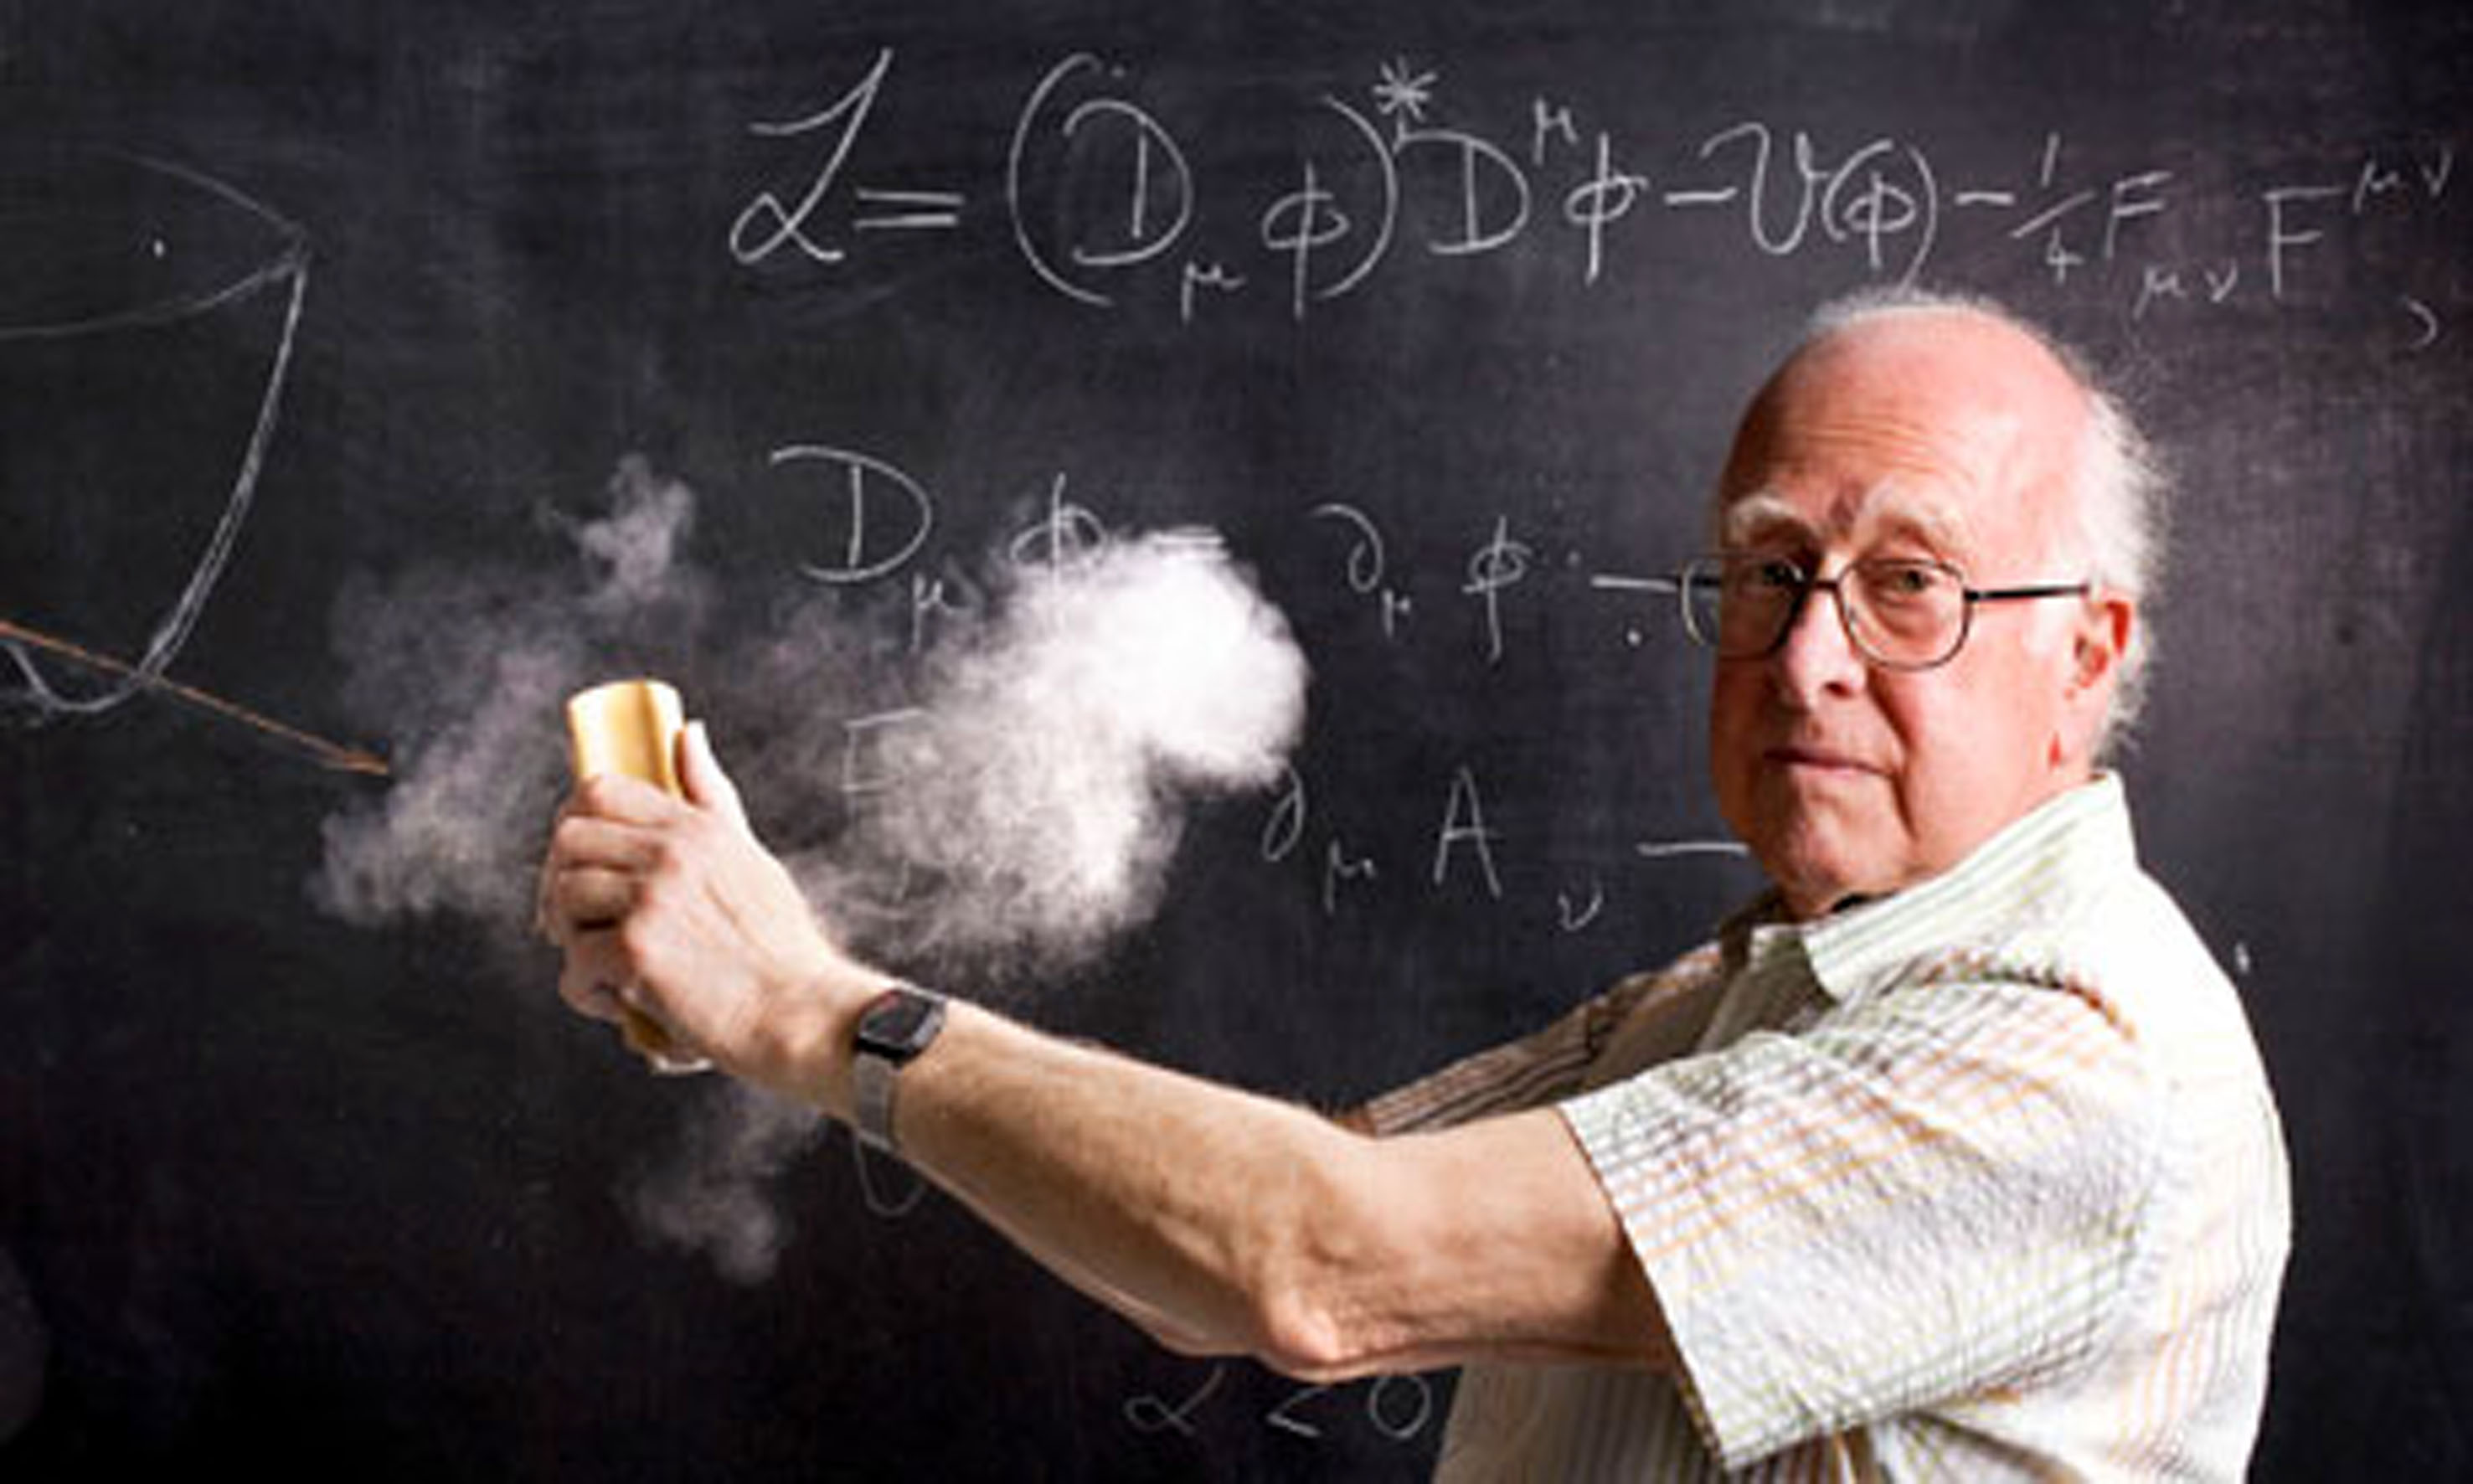
\includegraphics[scale=0.5]{images/Peter_Higgs.jpg}
\caption{Peter Higgs borrando la pizarra en la que est\'a escrita el lagrangiano del ahora llamado campo de Higgs y un campo de norma Abeliano.}
\end{figure}


\begin{figure}
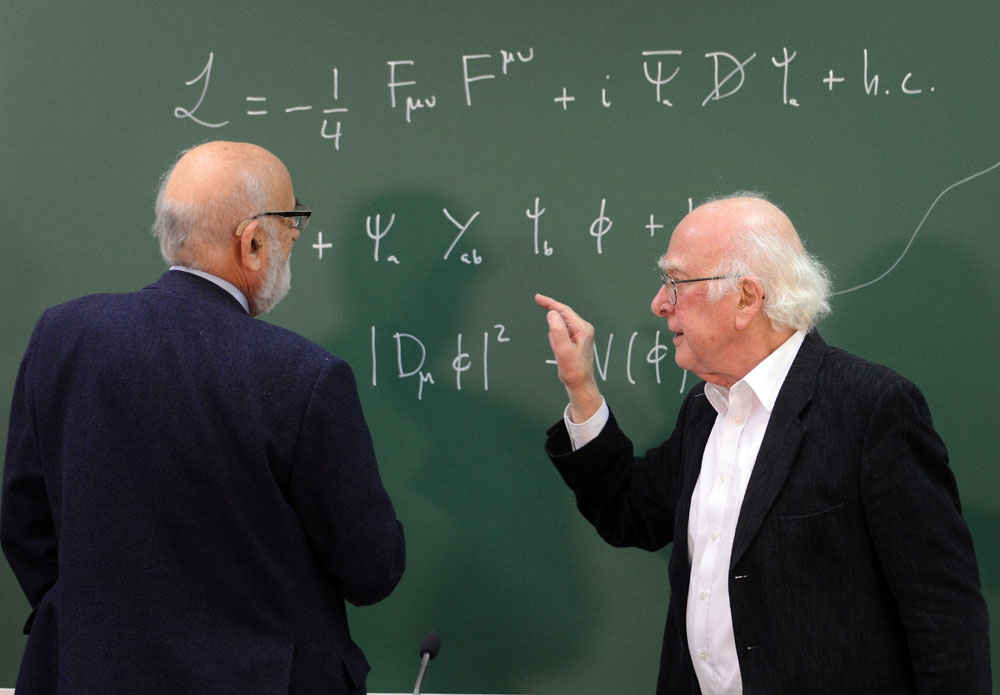
\includegraphics[scale=0.5]{images/higgs_englert_pizarra.jpeg}
\caption{Peter Higgs y Francois Englert discutiendo en la pizarra en la que est\'a escrita el lagrangiano que involucra al ahora llamado campo de Higgs. ¿Qu\'e creen que Higgs le dice a Englert? ¿Ser\'a acaso algo relacionado a la segunda l\'inea?}
\end{figure}

\begin{figure}
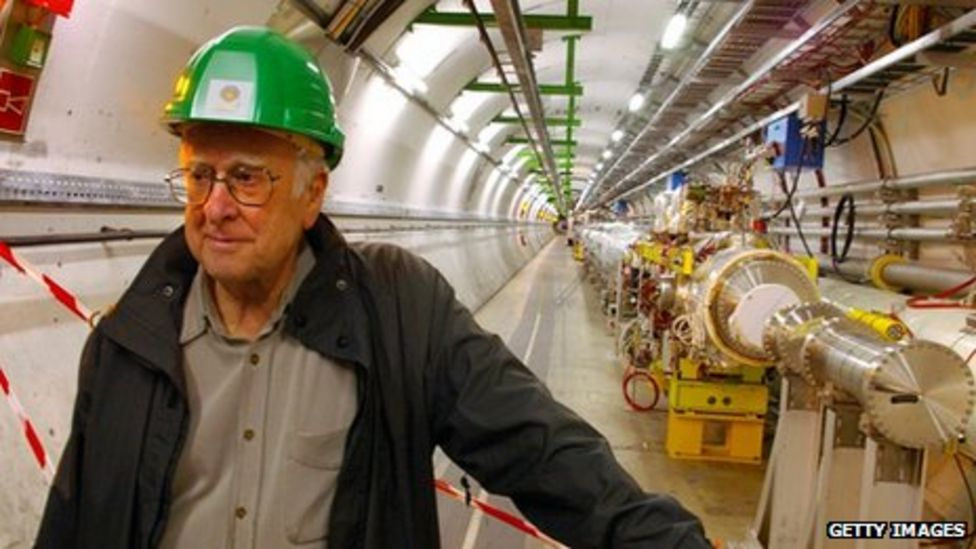
\includegraphics[scale=0.5]{images/higgs_lhc.jpg}
\caption{Peter Higgs en el LHC (Large Hadron Collider) del CERN.}
\end{figure}

\begin{figure}
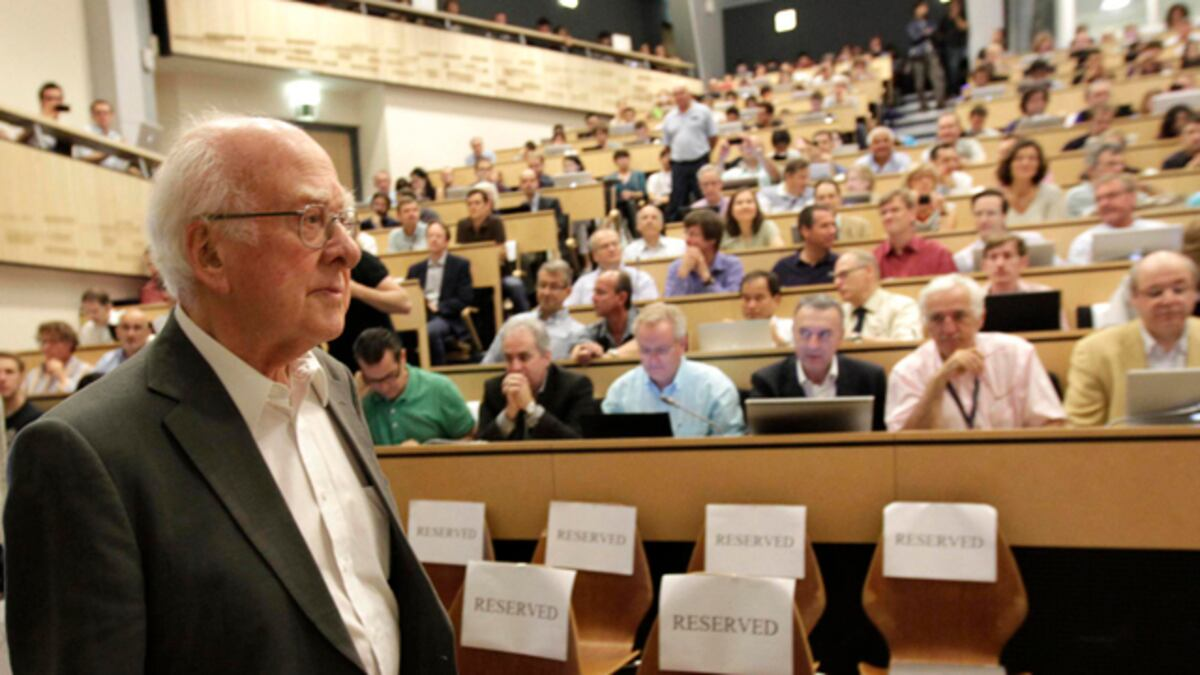
\includegraphics[scale=0.2]{images/higgs_anuncio.jpg}
\caption{El 4 de julio de 2012 el CERN hizo p\'ublico el descubrimiento del bos\'on de Higgs. Peter Higgs conmovido hasta las l\'agrimas en la ceremonia dijo: ``Felicitaciones a todos los involucrados en este descubrimento. Para m\'i es algo verdaderamente incre\'ible que haya vivido para verlo''.}
\end{figure}

\begin{figure}
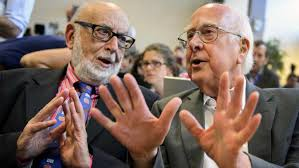
\includegraphics[scale=1]{images/higgs_englert.jpeg}
\caption{La Real Academia Sueca de las Ciencias otorg\'o el premio Nobel de F\'isica en 2013 a Francois Englert (izquierda) y a Peter Higgs (derecha) por ``el descubrimiento te\'orico de un mecanismo que contribuye a nuestra comprensi\'on del origen de la masa de las part\'iculas subat\'omicas...''}
\end{figure}

\begin{figure}
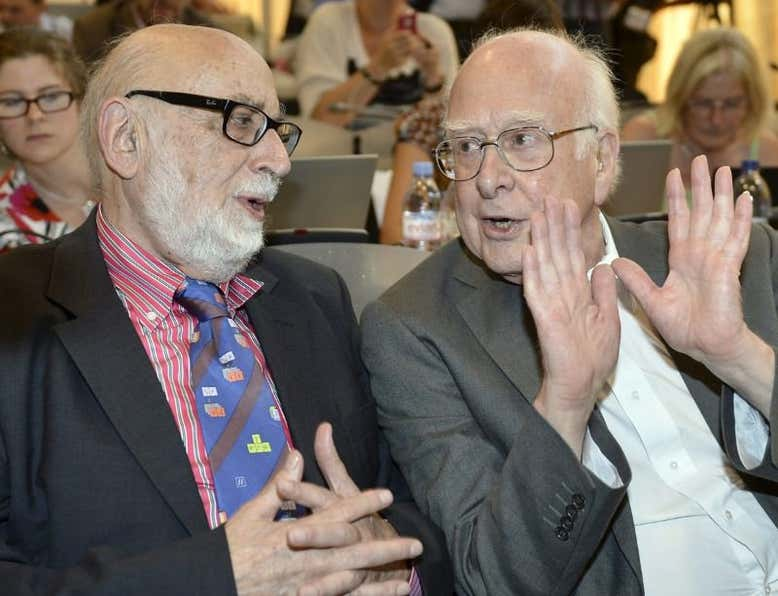
\includegraphics[scale=0.5]{images/higgs_englert2.jpeg}
\caption{La Real Academia Sueca de las Ciencias otorg\'o el premio Nobel de F\'isica en 2013 a Francois Englert (izquierda) y a Peter Higgs (derecha) por ``el descubrimiento te\'orico de un mecanismo que contribuye a nuestra comprensi\'on del origen de la masa de las part\'iculas subat\'omicas...''}
\end{figure}

\begin{figure}
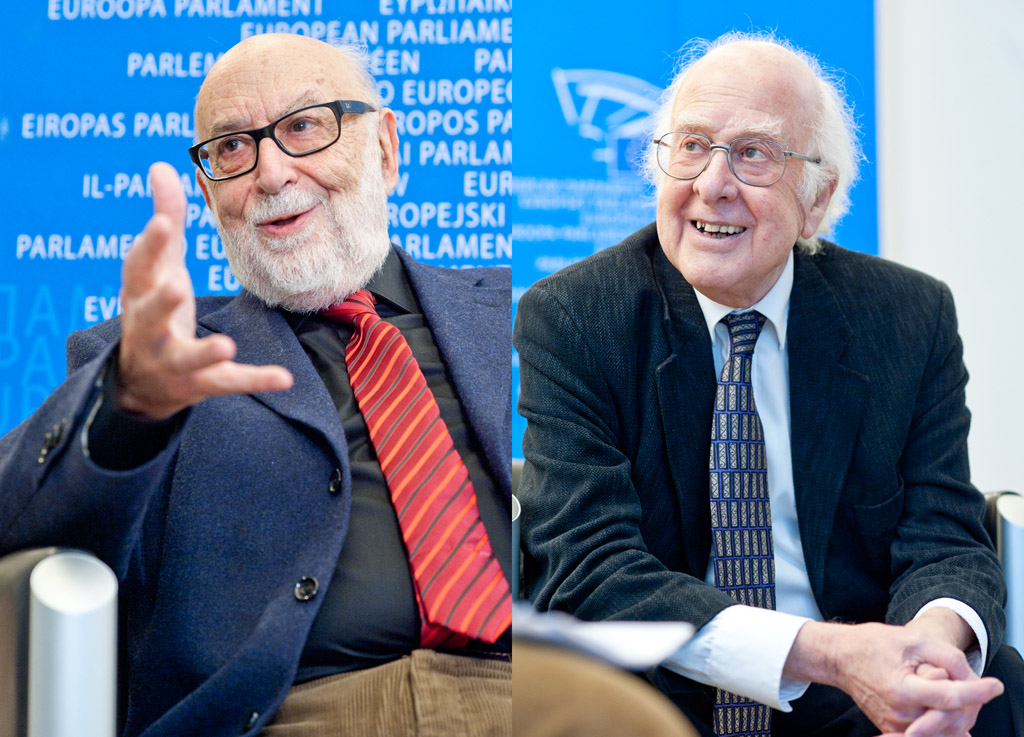
\includegraphics[scale=1]{images/higgs_englert3.jpeg}
\caption{La Real Academia Sueca de las Ciencias otorg\'o el premio Nobel de F\'isica en 2013 a Francois Englert (izquierda) y a Peter Higgs (derecha) por ``el descubrimiento te\'orico de un mecanismo que contribuye a nuestra comprensi\'on del origen de la masa de las part\'iculas subat\'omicas...''}
\end{figure}

\begin{figure}
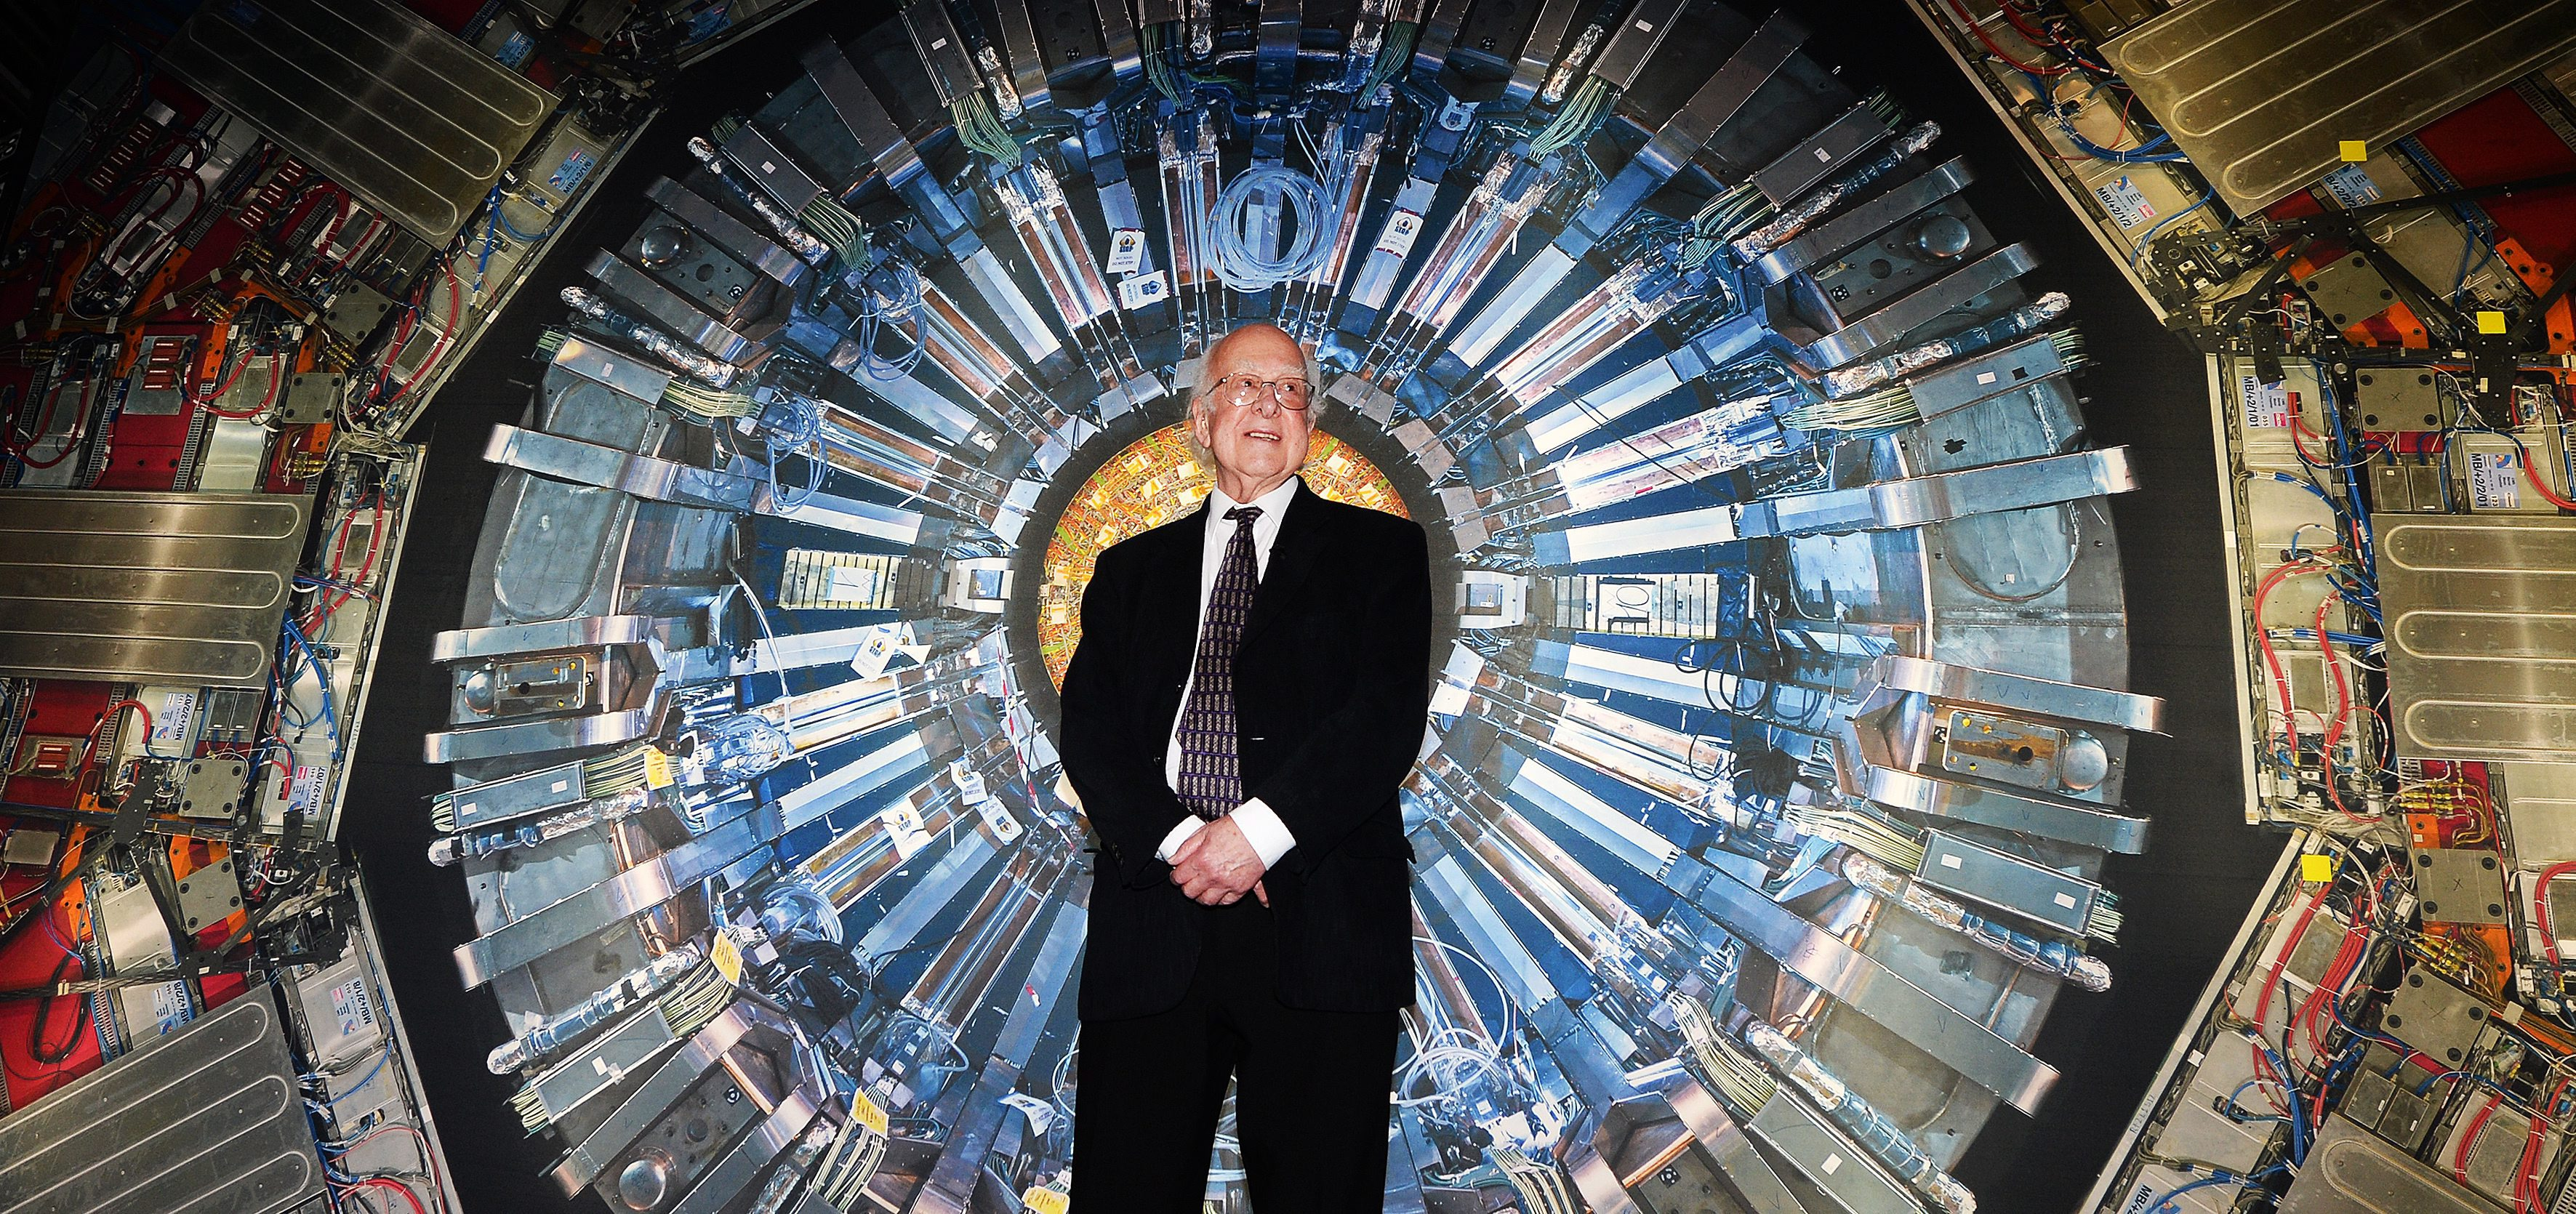
\includegraphics[scale=0.5]{images/higgslhc2.jpg}
\caption{Peter Higgs junto a una imagen del detector ATLAS del CERN. ATLAS es un detector multiprop\'osito usado para colisiones entre part\'iculas de muy alta energ\'ia. Particularmente, se usa para medir la masa, el momento, energ\'ia, carga el\'ectrica y esp\'in de estas part\'iculas.}
\end{figure}


\begin{figure}
	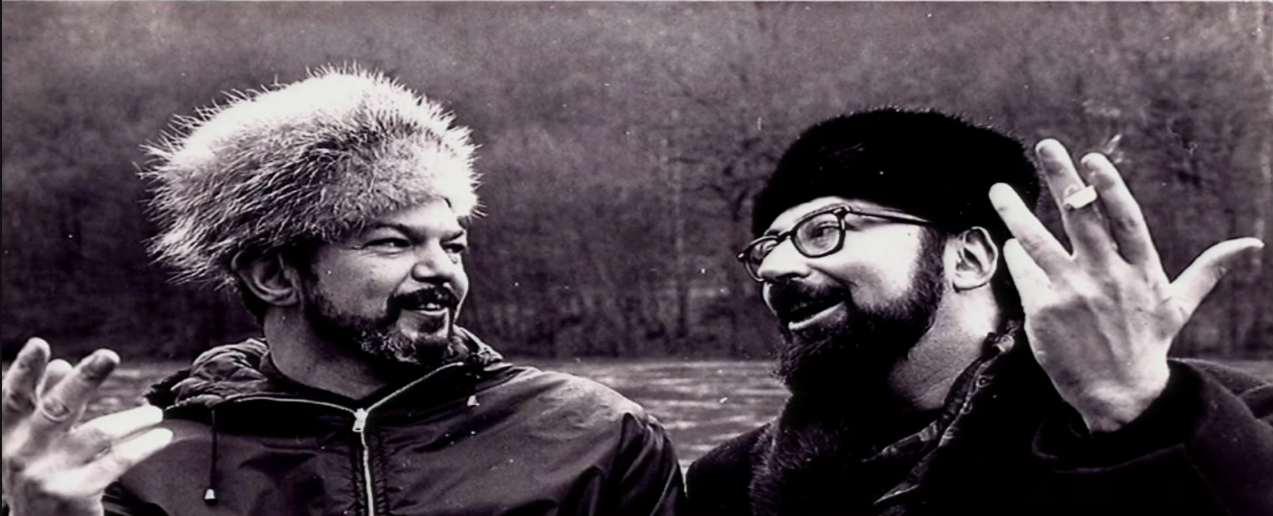
\includegraphics[scale=0.3]{images/brout_englert.png}
	\caption{Robert Brout (izquierda) y Francois Englert (derecha). Brout invit\'o a Englert a trabajar en la universidad de Cornell en 1959 por dos años como investigador asociado. Despu\'es de estos dos años Brout y Englert dejaron Cornell para trabajar en la Universidad de Bruselas, B\'elgica. Solo a Englert y Higgs les fue otorgado el premio Nobel en 2013, ya que Brout hab\'ia muerto en 2011.}
\end{figure}

\begin{figure}
\begin{subfigure}{0.3\textwidth}
	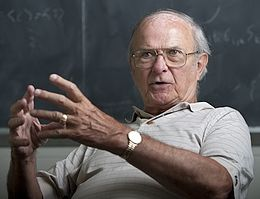
\includegraphics[scale=2]{images/hagen.jpg}
\end{subfigure}	
\begin{subfigure}{0.3\textwidth}
	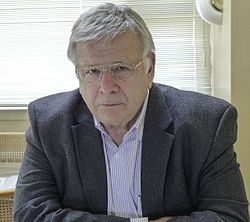
\includegraphics[scale=0.5]{images/guralnik.jpg}
\end{subfigure}	
\begin{subfigure}{0.3\textwidth}
	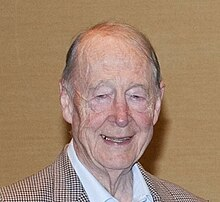
\includegraphics[scale=0.5]{images/kibble.jpg}
\end{subfigure}	

	\caption{Los otros descubridores del mecanismo de Higgs. De izquierda a derecha, Carl Hagen, Gerald Guralnik y Tom Kibble. De manera controversial ellos fueron excluidos del premio Nobel en 2013.} 
\end{figure}

	\begin{figure}
	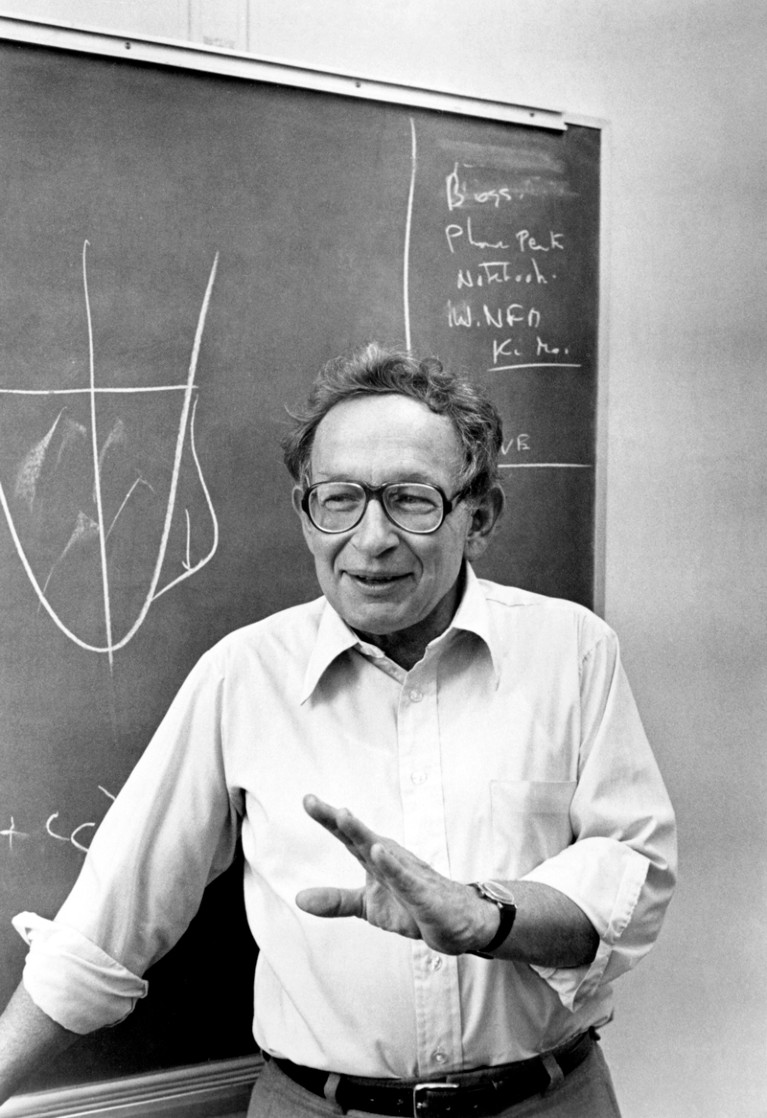
\includegraphics[scale=0.3]{images/anderson.jpg}
	\caption{Philip Anderson descubri\'o el mecanismo que da masa a los bosones de norma en el contexto de materia condensada. Fue galardonado con el premio Nobel de f\'isica en 1977.}
	\end{figure}
	
	\begin{figure}
	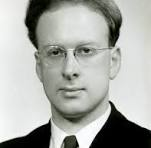
\includegraphics[scale=1]{images/higgs_joven.jpeg}
	\caption{Peter Higgs solo public\'o dos art\'iculos sobre el tema en 1964 y 1966.}
	\end{figure}
	
\begin{figure}
\begin{subfigure}{0.5\textwidth}
	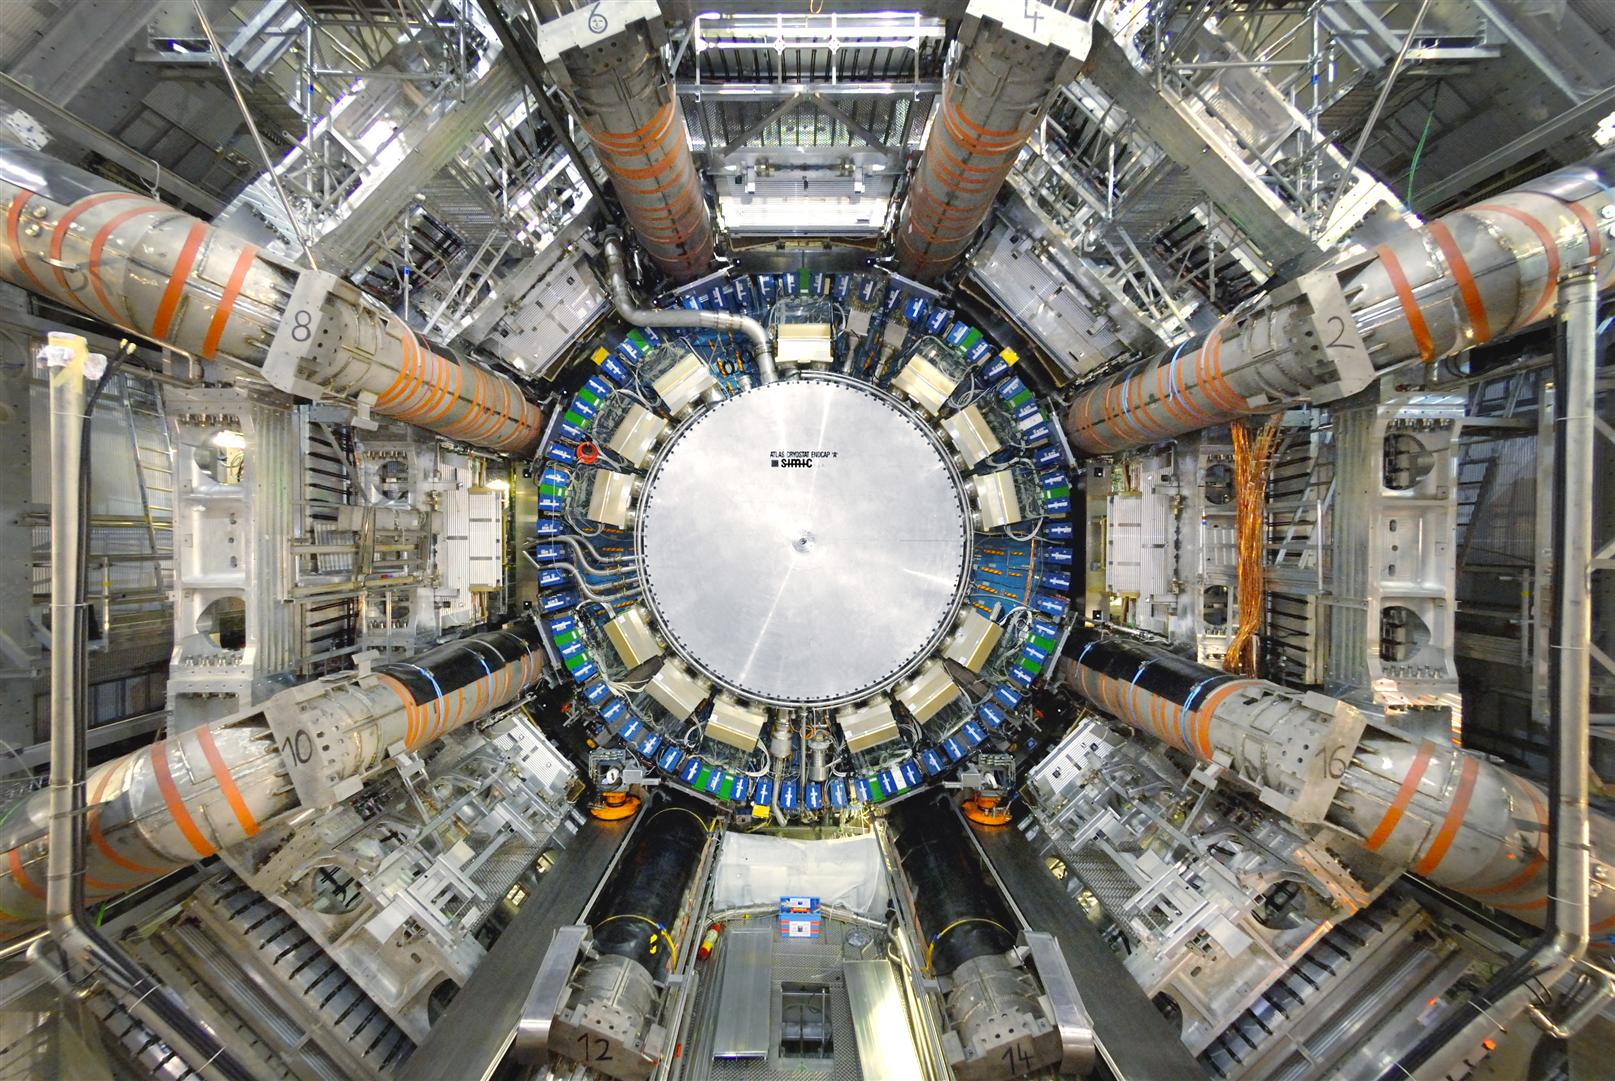
\includegraphics[scale=0.27]{images/atlas.jpg}
\end{subfigure}	
\begin{subfigure}{0.5\textwidth}
	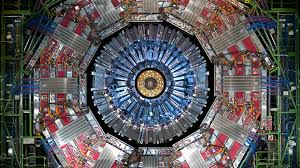
\includegraphics[scale=0.9]{images/cms.jpeg}
\end{subfigure}	
\caption{Detector ATLAS (izquierda) y el detector CMS (derecha) en el CERN fueron los que confirmaron las existencia del bos\'on de Higgs del Modelo Est\'andar. Tanto ATLAS y CMS son detectores multiprop\'osito usados para analizar colisiones entre part\'iculas de muy alta energ\'ia.}
\end{figure}


\begin{figure}
\begin{subfigure}{0.5\textwidth}
	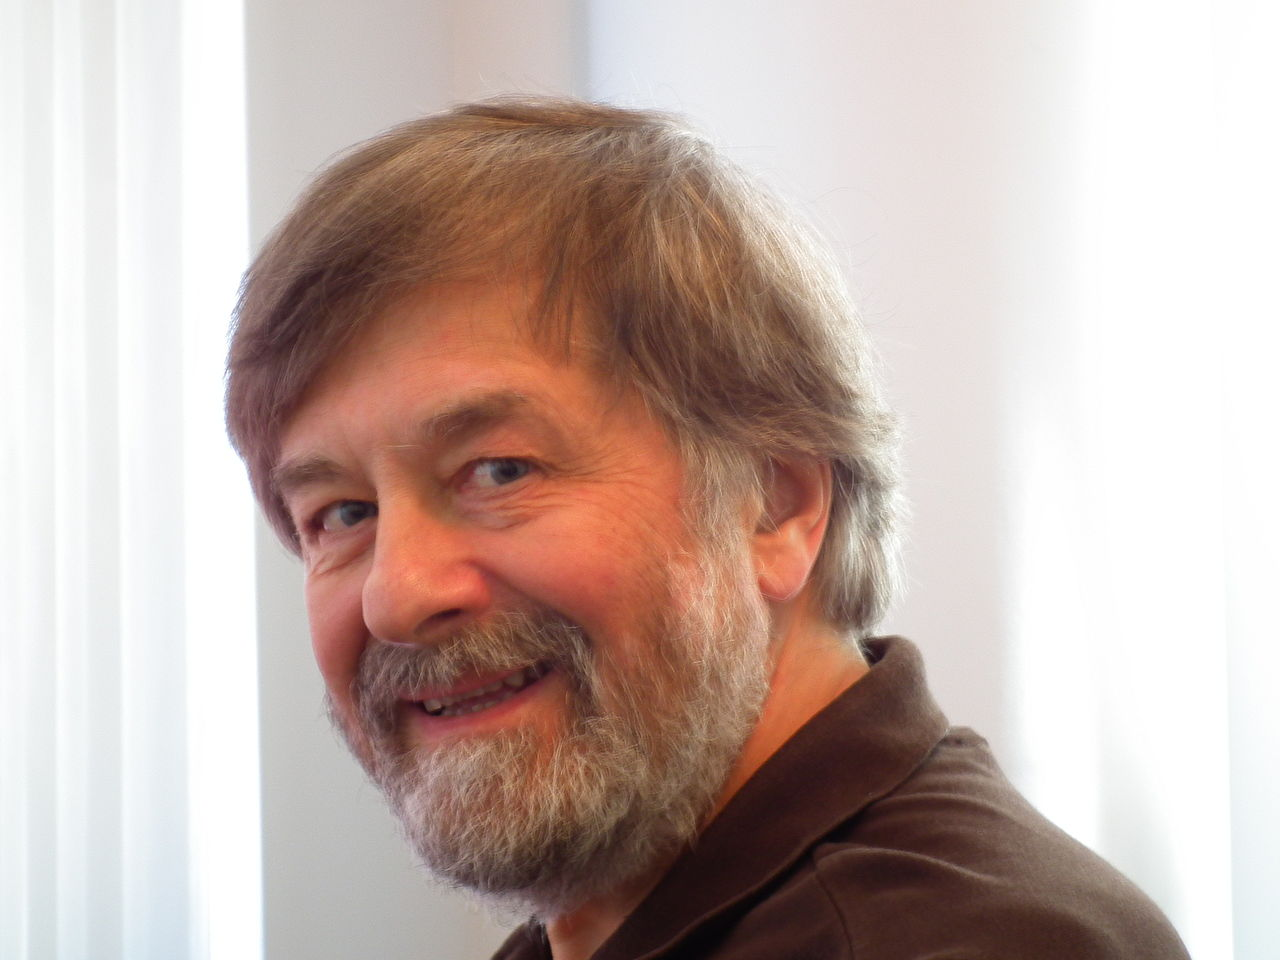
\includegraphics[scale=0.18]{images/migdal.jpg}
\end{subfigure}	
\begin{subfigure}{0.5\textwidth}
	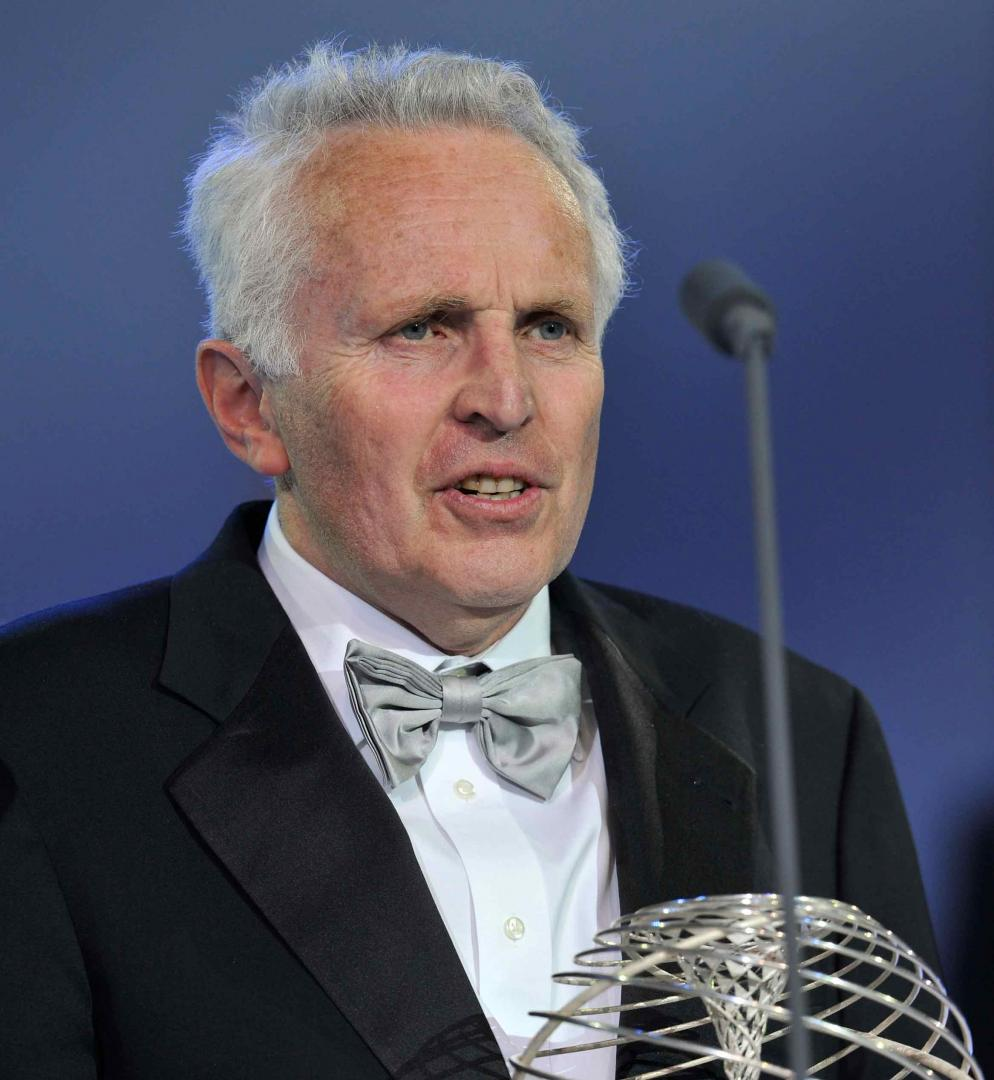
\includegraphics[scale=0.15]{images/polyakov.jpg}
\end{subfigure}	
\caption{Cuando a\'un eran estudiantes de licenciatura Alexander Migdal (izquierda) y Alexander Polyakov (derecha) desarrollaron de manera conjunta e independiente de Higgs y otros sobre los efectos del rompimiento espont\'aneo de una simetr\'ia de norma y c\'omo da lugar a la masa de los bosones de norma.}
\end{figure}


\begin{figure}
\begin{subfigure}{0.5\textwidth}
	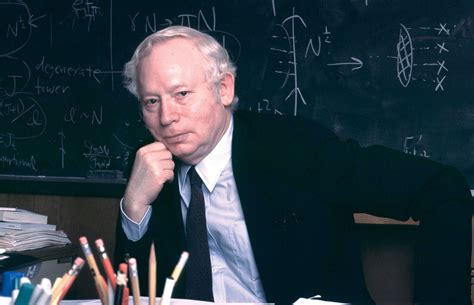
\includegraphics[scale=0.5]{images/weinberg.jpeg}
\end{subfigure}	
\begin{subfigure}{0.5\textwidth}
	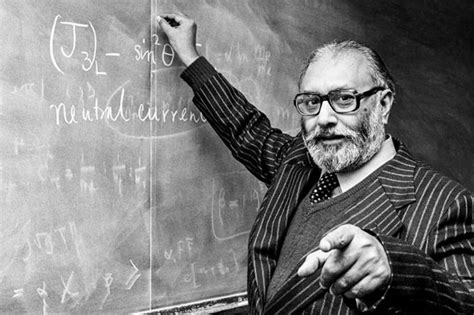
\includegraphics[scale=0.5]{images/salam.jpeg}
\end{subfigure}	
\caption{Steven Weinberg (izquierda) y Abdus Salam (derecha) independientemente integraron el mecanismo de Higgs al sector electrod\'ebil. Ambos compartieron el premio Nobel de f\'isica en 1979 junto a Sheldon Glashow.}
\end{figure}

\end{document}